\documentclass{article}
\usepackage{amsmath}
\usepackage{graphicx}
\usepackage{hyperref}
\usepackage{enumitem}
\usepackage{float}
\usepackage{wrapfig}
\usepackage{parskip}


\usepackage[a4paper, total={6in, 8in}]{geometry}

\title{Notes on Auditory Perception and Neural Processing}
\author{}
\date{}

\begin{document}

\maketitle

\newpage

\tableofcontents

\newpage

\section{Acronyms}

\begin{tabbing}
    \textbf{Acronym} \hspace{3cm} \= \textbf{Stands for} \\
    ANN \> Artificial Neural Network \\
    ASSR \> Auditory Steady-State Response \\
    BWE \> Brain Wave Entrainment \\
    EEG \> Electroencephalogram \\
    FFR \> Frequency Following Response \\
    HRTF \> Head-related Transfer Function \\
    HT \> Hilbert Transform \\
    ITD \> Interaural Time Differences \\
    KAN \> Kolmogorov-Arnold Networks \\
    LSTM \> Long-Short Term Memory \\
    MFCC \> Mel Frequency Cepstral Coefficient \\
    MPL \> Multi-Layer Perceptrons \\
    MSO \> Medial Superior Olive \\
    PLV \> Phase Locking Value \\
    RNN \> Recurrent Neural Network \\
    SSD \> Singular Spectrum Decomposition \\
    TE \> Transfer Entropy \\
    TWCO \> Theory of Weakly Coupled Oscillators \\
\end{tabbing}

\newpage

\section{Neural Basis}
Outside of the cochlea, dendrites of the spiral ganglion cells synapse with the base of the hair cells located in the organ of Corti on the basilar membrane. 

\begin{wrapfigure}{r}{0.5\textwidth}  % 'r' for right, and set the width of the figure
\centering
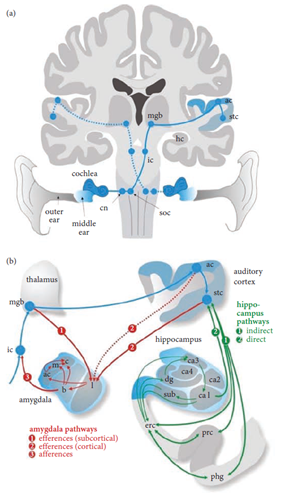
\includegraphics[width=0.5\textwidth]{pathways.png}  % Adjust the width
\caption{Anatomy of the auditory pathway.}
\label{fig:auditory-pathway}
\end{wrapfigure}

Triggered by the movement of the hair cells on the basilar membrane, the spiral ganglion cells are the first neurons to fire an action potential in the auditory pathway, transmitting all the brain's auditory input via their axons synapsing with the dendrites of the cochlear nuclei. The majority of the fibers (70 percent) cross over to the opposite hemisphere starting at the levels of the cochlear nuclei (contralateral pathway), while some remain on the same incoming side (ipsilateral pathway). The acoustic information is highly preprocessed by a series of brainstem nuclei before reaching the cortex. Basic acoustic features such as sound intensity, signal onsets, periodicity, and signal location are extracted in the cochlear nucleus, lateral lemniscus, and the superior olivary complex. There is a secondary pathway that originates in the ventral cochlear nucleus where some fibers project from there to the reticular formation, a general arousal system in the lower brainstem. Descending (efferent) fiber tracts from the reticular formation form the audio-spinal pathway by connecting with the motor neurons in the spinal cord to innervate reflexive motor responses to sound and to prime motor neural excitability. The secondary ascending (afferent) pathway inhibits lower auditory centers to elevate hearing thresholds and alert the cortex to incoming auditory signals.
In the primary ascending pathway, the superior olivary complex is the first relay station of the brainstem where cochlear inputs from both left and right sides converge, providing the anatomical basis for the processing of sound location by measuring timing and sound intensity differences between incoming left and right signals to determine sound angles (Grothe, 2000; Tollin, 2003). More complex spectral and temporal decoding of the acoustic signals occurs in the inferior colliculus. Functional magnetic resonance imaging research with animals has shown that the spectral and temporal dimensions of the acoustic signals are distinctly mapped in the inferior colliculus, indicating that, in addition to the tonotopic maps, the temporal envelope of the acoustic signals are also topographically represented in the inferior colliculus (Baumann et al., 2011, 2015; Mei et al., 2013). The last cross-lateral projections are at the inferior colliculus level.
The last subcortical node in the primary ascending pathway is the medial geniculate body, which is comprised of multiple subdivisions. The ventral nucleus of the medial geniculate body is tonotopically organized and is the main ascending route to the primary auditory cortex, while its other subdivisions project widely to both primary and non-primary auditory cortex. Importantly, the auditory pathway does not only consist of ascending projections; it also has rich top-down projections that are critical for modulation of neural responses in the subcortical auditory centers and for learning-induced plasticity (Bajo et al., 2010; Suga \& Ma, 2003). \textbf{In general, conduction in the auditory pathway is faster and stronger for the contralateral pathway}.


\subsection{Cochlea and Spiral Ganglion Cells}
    \textbf{Cochlea:} A spiral-shaped organ in the inner ear where sound vibrations are converted into neural signals. \\
    \textbf{Hair Cells:} Located in the organ of Corti on the basilar membrane, they move in response to sound vibrations. \\
    \textbf{Spiral Ganglion Cells:} The dendrites of these cells synapse with the base of the hair cells. Movement of the hair cells triggers these ganglion cells to fire action potentials, marking the first neural response in the auditory pathway.
    
\subsection{Pathway to the Brainstem}
    \textbf{Cochlear Nuclei:} The axons of the spiral ganglion cells transmit auditory information to the cochlear nuclei in the brainstem. Here fibers can follow either a contralateral or ipsilateral pathway: \\
    \textbf{Contralateral Pathway:} The majority (70\%) of fibers cross to the opposite hemisphere. \\
    \textbf{Ipsilateral Pathway:} Some fibers remain on the same side.
    
\subsection{Brainstem Processing}
\textbf{Cochlear Nucleus, Lateral Lemniscus, and Superior Olivary Complex:} These brainstem nuclei preprocess acoustic features such as sound intensity, signal onsets, periodicity, and signal location. \\
\textbf{Superior Olivary Complex:} The first relay station where inputs from both ears converge, processing sound location by measuring timing and intensity differences between the ears.

\subsection{Secondary Pathway and Reflexes}
\textbf{Ventral Cochlear Nucleus:} Some fibers project to the reticular formation, part of a general arousal system in the lower brainstem. \\
\textbf{Audio-Spinal Pathway:} Efferent fibers from the reticular formation connect with motor neurons in the spinal cord, enabling reflexive motor responses to sound.

\subsection{Advanced Processing in the Midbrain}
\textbf{Inferior Colliculus:} Involved in complex spectral and temporal decoding of sounds. Functional MRI studies show distinct mappings of spectral and temporal dimensions in addition to tonotopic maps.

\subsection{Thalamic Relay}
\textbf{Medial Geniculate Body:} The final subcortical relay station. The ventral nucleus is tonotopically organized and routes information to the primary auditory cortex. Other subdivisions project to both primary and non-primary auditory cortices.
\subsection{Auditory Cortex and Top-Down Modulation}
\textbf{Primary Auditory Cortex:} Receives the main input from the medial geniculate body. \\
\textbf{Top-Down Projections:} Rich descending pathways modulate neural responses in subcortical auditory centers and contribute to learning-induced plasticity.

\subsubsection{Key Points}
\begin{itemize}
    \item \textbf{Contralateral Dominance:} Conduction is faster and stronger for the contralateral pathway.
    \item \textbf{Topographic Representation:} Both spectral and temporal aspects of sounds are topographically mapped in the inferior colliculus.
\end{itemize}

\subsection{Interaural time differences}

A basic concept in neuroscience is to correlate specific functions with specific neuronal structures. By discussing a specific example, an alternative concept is proposed: structures may be linked to rules of processing and these rules may serve different functions in different species or at different stages of evolution. The medial superior olive (MSO), a mammalian auditory brainstem structure, has been thought to solely process interaural time differences (ITD), the main cue for localizing low frequency sounds. Recent findings, however, indicate that this is not its only function since mammals that do not hear low frequencies and do not use ITDs for sound localization also possess an MSO.


\section{Ohm’s Acoustic Law}
Ohm's acoustic law states that the human ear perceives complex sounds in terms of their constituent sinusoidal (pure tone) components. Essentially, the ear performs a kind of Fourier analysis, breaking down complex auditory signals into simpler sinusoidal waves, each with its own frequency, amplitude, and phase.

\subsection{Key Aspects of Ohm's Acoustic Law}

\subsubsection{Frequency Resolution:}
According to Ohm's law of acoustics, the ear can resolve and identify the different frequencies present in a complex sound. This is akin to recognizing the individual notes in a chord played on a piano.

\subsubsection{Harmonic Analysis:}
The auditory system analyzes harmonic sounds by detecting the individual harmonics or overtones that make up the sound. This allows the brain to perceive the pitch and timbre of complex sounds, even if the fundamental frequency is not physically present (as in the case of the \textit{missing fundamental}).

\subsubsection{Spectral Components:}
The perception of sound is largely determined by the spectral components (the individual frequencies) rather than the phase relationships between them. This means that the ear is more sensitive to the frequency content of a sound than to the specific timing (phase) of the waveforms.


\section{Seebeck's Periodicity Theory}

\textit{Seebeck} proposed that the perception of pitch is based on the periodicity (repetition rate) of a sound wave rather than its harmonic content. This contrasts with the spectral theories of pitch perception, which emphasize the importance of individual frequency components.

According to \textit{Seebeck}, the auditory system detects the temporal pattern of the sound wave. The periodic repetition of the waveform, regardless of its harmonic structure, determines the perceived pitch.

\textit{Seebeck} conducted experiments with complex tones and found that listeners could perceive a fundamental pitch even when the fundamental frequency was absent, as long as the periodicity of the waveform suggested that pitch. This phenomenon is related to the concept of the \textbf{Missing fundamental}.

\textit{Seebeck}'s work influenced later theories of pitch perception, including the temporal theory of pitch perception, which emphasizes the role of timing and \textbf{phase-locking} in auditory neurons.

Contemporary models recognize that both the temporal pattern (periodicity) and the harmonic content (spectral information) contribute to pitch perception. This integrated approach is supported by findings in auditory neuroscience and psychoacoustics.

\section{Missing fundamental}

When a sound consists of a series of harmonics (integer multiples of a base frequency) without the actual base frequency (fundamental) being present, the brain perceives the pitch corresponding to that base frequency.

\textbf{Example:} If a sound contains harmonics at 300 Hz, 400 Hz, and 500 Hz, the fundamental frequency would be 100 Hz (the greatest common divisor of the harmonic frequencies). Even though 100 Hz is not physically present in the sound, listeners perceive the pitch as if it were.


\subsection{Missing Fundamental}
When a sound consists of a series of harmonics (integer multiples of a base frequency) without the actual base frequency (fundamental) being present, the brain perceives the pitch corresponding to that base frequency.

\textbf{Example:} If a sound contains harmonics at 300 Hz, 400 Hz, and 500 Hz, the fundamental frequency would be 100 Hz (the greatest common divisor of the harmonic frequencies). Even though 100 Hz is not physically present in the sound, listeners perceive the pitch as if it were.

\section{Auditory Steady-State, Frequency-Following Responses}
    
\subsection{Auditory Steady-State Responses (ASSR)}
ASSRs are a type of neural response to auditory stimuli characterized by the brain's ability to synchronize its electrical activity with the rhythm of the stimulus. When binaural beats are presented, the brain's electrical activity can lock onto the beat frequency, demonstrating an ASSR. This synchronization occurs at the cortical level and reflects the brain's capacity to follow the repetitive auditory stimulus, which in the case of binaural beats, is the frequency difference between the two tones presented to each ear.

\subsection{Frequency-Following Responses (FFR)}
FFRs are neural responses that occur at the subcortical level, specifically in the brainstem. These responses indicate the brainstem's ability to follow the frequency changes in the auditory stimuli. For binaural beats, the FFRs demonstrate that the brainstem can track the frequency difference between the two tones, which is perceived as the binaural beat. This response is crucial for understanding how binaural beats are processed early in the auditory pathway before the information is relayed to higher cortical areas.

\subsubsection{Key Points from the Paper Orozco Perez et al. (2020)}
\begin{itemize}
    \item \textbf{Entrainment at Different Levels:} Both ASSRs and FFRs are elicited by binaural beats, indicating that these beats can entrain brain activity at both cortical and subcortical levels. ASSRs represent cortical entrainment, while FFRs represent subcortical (brainstem) entrainment.
    \item \textbf{Functional Connectivity:} The study also explores changes in functional connectivity patterns in the brain induced by binaural beats. Functional connectivity refers to the temporal correlation between spatially remote neurophysiological events. The findings suggest that binaural beats can alter connectivity patterns, potentially influencing cognitive and emotional states.
    \item \textbf{Subjective Effects:} The paper examines subjective reports of mood changes in response to binaural beats, linking these subjective experiences with objective neural measures (ASSRs and FFRs). For example, theta beats (around 7 Hz) are associated with relaxation, while gamma beats (around 40 Hz) are linked to heightened alertness and attention.
\end{itemize}

\section{Generating Brain Waves}
Synchronization of neuronal activity in the brain underlies the emergence of neuronal oscillations, termed brain waves, which serve various physiological functions and correlate with different behavioral states. At least ten distinct mechanisms are involved in the generation of brain waves, including variations in the concentration of extracellular neurotransmitters and ions, as well as changes in cellular excitability.

In this context, astrocytes—a subtype of glial cells—play an important role in the formation and modulation of brain waves. Their close association with synapses allows bidirectional interaction with neurons, and their syncytium-like activity via gap junctions facilitates communication to distant brain regions through Ca\(^2+\) waves.

\subsection{Key Functions of Astrocytes}
\begin{itemize}
    \item \textbf{Regulation of Neuronal Excitability:} Astrocytes regulate neuronal excitability via glutamate uptake and tight control of extracellular K\(^+\) levels through a process known as K\(^+\) clearance.
    \item \textbf{Synaptic Plasticity:} Astrocytes also contribute to learning and memory by modulating synaptic plasticity through their interaction with neurons.
\end{itemize}

\section{Binaural Auditory Stimuli}
Binaural auditory stimuli involve presenting two slightly different frequencies to each ear, which the brain processes as a single tone. This process results in a perception known as binaural beats, which have been shown to influence brain wave activity and induce states of relaxation or focus.

According to research, brain and body signals oscillate in synchrony, aligning with each other to form a "single frequency architecture." This interaction can be described using the equation:
\[
fd(i) = s \times 2^i
\]
where $s$ is the scaling factor, $i$ refers to the biosignal of interest, and $f$ is the fundamental frequency of the biosignal oscillation. When $i = 0$, $f_d$ refers to cardiac activity. When $i < 0$, $f_d$ refers to breathing rhythms (including Mayer waves that are the lowest frequency in the respiratory process), blood pressure waves, rhythmic fluctuations in the blood oxygen level-dependent (BOLD) signal at intrinsic mode fluctuations, and gastric waves. 

When $i > 0$, $f_d$ refers to brain oscillations [delta ($i = 1$), theta ($i = 2$), alpha ($i = 3$), beta ($i = 4$), gamma ($i = 5$)].

In addition, upper and lower frequencies of each fundamental frequency can be, respectively, estimated by:

\[
uf_b(i) = \frac{1.25 \cdot 2^{i+1}}{g}
\]

\[
lf_b(i) = (1.25 \cdot 2^{i-1}) \cdot g
\]
\section{Phase Oscillator Models}

These models, based on the Theory of Weakly Coupled Oscillators (TWCO), are effective for simulating phase synchronization dynamics. 

Phase-oscillator models have been used to simulate synchronization in neural networks, showing that they can replicate the phase-locking behaviors observed in real neural data.

Synchronization, or phase-locking, between oscillating neuronal groups is considered to be important for the coordination of information among cortical networks. \textbf{Spectral coherence} is a commonly used approach to quantify phase-locking between neural signals. We systematically explored the validity of spectral coherence measures for quantifying synchronization among neural oscillators. To that aim, we simulated coupled oscillatory signals that exhibited synchronization dynamics using an abstract phase-oscillator model, as well as interacting gamma-generating spiking neural networks. 

We found that, within a large parameter range, the spectral coherence measure deviated substantially from the expected phase-locking. Moreover, spectral coherence did not converge to the expected value with increasing signal-to-noise ratio. We found that spectral coherence particularly failed when oscillators were in the partially (intermittent) synchronized state, which we expect to be the most likely state for neural synchronization. This failure was due to the fast frequency and amplitude changes induced by synchronization forces.

We then investigated whether spectral coherence reflected the information flow among networks, measured by \textbf{transfer entropy (TE)} of spike trains. We found that spectral coherence failed to robustly reflect changes in synchrony-mediated information flow between neural networks in many instances. As an alternative approach, we explored a \textbf{phase-locking value (PLV)} method based on the reconstruction of the instantaneous phase. One approach for reconstructing instantaneous phase is the \textbf{Hilbert Transform (HT)} preceded by \textbf{Singular Spectrum Decomposition (SSD)} of the signal

PLV estimates have broad applicability as they do not rely on stationarity and, unlike spectral coherence, they enable more accurate estimations of oscillatory synchronization across a wide range of different synchronization regimes and better tracking of synchronization-mediated information flow among networks \cite{Lowet2016}.

PLV is preferred over traditional spectral coherence for neural synchronization because it better handles non-stationary dynamics and provides a clearer measure of phase consistency \cite{Schmidt2014}.


\subsection{Synchronization}
Synchronization, or phase-locking, between oscillating neuronal groups is considered important for the coordination of information among cortical networks. Spectral coherence is commonly used to quantify phase-locking between neural signals. Simulations of coupled oscillatory signals demonstrate the effectiveness of this approach.

\textbf{Kuramoto Model:} The Kuramoto model is a widely used mathematical model for describing synchronization phenomena in systems of coupled oscillators. It’s used to study neural synchronization, circadian rhythms, and more.

\section{Rhythmic Entrainment in Music}
Rhythmic entrainment refers to the synchronization of brain activity to an external rhythmic stimulus, like music. Studies show that repetitive rhythmic patterns can entrain neural oscillations, influencing cognitive and emotional states.

\subsection{Repetitive Rhythmic Music, EEG, and Subjective Experience}
Jilek observed a predominance in drumming frequencies at 4 to 7 beats per second—a range that correlates with the theta wave frequency band (4–7 Hz) of the human EEG. Stimulation in this frequency range is believed to aid in entering altered states of consciousness, such as ecstasy and creativity.

\section{Artificial Neural Networks}
Artificial Neural Networks (ANNs) are computational models inspired by biological neural networks. They consist of layers of interconnected nodes (neurons) that process input data.

\subsection{Kolmogorov-Arnold Networks (KAN)}
Kolmogorov-Arnold Networks (KANs) are a type of ANN based on the Kolmogorov-Arnold representation theorem. They eliminate the need for linear weight matrices and use learnable activation functions on the edges.

\subsubsection{Key Differences from Multi-Layer Perceptrons (MLPs)}
\begin{itemize}
    \item \textbf{No Linear Weights:} KANs do not require linear weights as MLPs do.
    \item \textbf{Learnable Activation Functions on Edges:} Instead of fixed activation functions on nodes (like ReLU), KANs have learnable activation functions on the edges.
    \item \textbf{Summation on Nodes:} Nodes in KANs simply sum the incoming signals without applying additional nonlinearities.
\end{itemize}

\subsubsection{Advantages of KANs}
\begin{itemize}
    \item \textbf{Accuracy:} KANs have demonstrated superior accuracy in tasks involving low-dimensional functions or compositional structures.
    \item \textbf{Interpretability:} KANs are more interpretable than MLPs due to their learnable activation functions and simpler structure.
    \item \textbf{Scientific Discovery:} KANs have been applied to rediscover mathematical relationships and physical laws.
\end{itemize}

\subsubsection{Training and Simplification}
KANs can be trained using backpropagation techniques, and methods such as L1 regularization and entropy regularization can encourage sparsity, making the network smaller and more interpretable.
\section{Gemini Dixit}
\subsection{Topology}
\begin{itemize}
    \item \textbf{Convolutional Neural Network (CNN):} CNNs capture spatial relationships between frequencies, which is crucial for binaural beat perception. 
    \item \textbf{Recurrent Neural Network (RNN) or Long Short-Term Memory (LSTM):} After initial CNN processing, an RNN or LSTM layer can capture the temporal relationship between sounds.
    \item \textbf{Output Layer:} The final layer predicts the perceived binaural beat frequency or desired effect, such as relaxation or focus.
\end{itemize}

\subsection{Transduction}
\textbf{Preprocessing:} Implement a Mel-frequency cepstral coefficient (MFCC) filter bank on the raw audio data. MFCCs mimic the human auditory system’s frequency response, focusing on perceptually relevant features.

\subsection{Additional Considerations}
\textbf{Head-Related Transfer Function (HRTF):} The model can incorporate HRTFs, which describe how sound interacts with the head and torso, affecting sound localization.

\subsection{Challenges}
Training the model requires a large dataset of binaural beats with well-defined characteristics and corresponding user responses. Obtaining high-quality HRTF data for a diverse population can be challenging.

\section{Kuramoto Model}
The Kuramoto model is a mathematical model used to describe synchronization phenomena in systems of coupled oscillators. Developed by Yoshiki Kuramoto in 1975, it explains how independent oscillators synchronize through weak interactions.

\subsection{Mathematical Formulation}
Each oscillator is represented by its phase, \(\theta_i(t)\), which evolves over time. The dynamics are governed by the equation:
\[
\frac{d\theta_i}{dt} = \omega_i + \frac{K}{N} \sum_{j=1}^{N} \sin(\theta_j - \theta_i)
\]
where:
\begin{itemize}
    \item \(\theta_i(t)\) is the phase of the \(i\)-th oscillator at time \(t\),
    \item \(\omega_i\) is the natural frequency of the \(i\)-th oscillator,
    \item \(K\) is the coupling constant,
    \item \(N\) is the number of oscillators.
\end{itemize}

\subsection{Synchronization}
When \(K\) is low, the oscillators behave independently. As \(K\) increases, oscillators begin to synchronize, aligning their phases. If \(K\) is large enough, complete synchronization occurs.

\section{Bibliography}
\begin{itemize}
    \item Bajo, V. M., Nodal, F. R., Moore, D. R., \& King, A. J. (2010). The descending corticocollicular pathway mediates learning-induced auditory plasticity. Nature Neuroscience, 13(2), 253–260.
    \item Baumann, S., Griffiths, T. D., Sun, L., Petkov, C. I., Thiele, A., \& Rees, A. (2011). Orthogonal representation of sound dimensions in the primate midbrain. Nature Neuroscience, 14(4), 423–425.
    \item Buzsáki, G. (2009). Rhythms of the Brain. Rhythms of the Brain. Oxford University Press.
    \item Orozco Perez, H. D., Dumas, G., \& Lehmann, A. (2020). Binaural beats through the auditory pathway: From brainstem to connectivity patterns. ENeuro, 7(2).
    \item Schmidt, B. T., Ghuman, A. S., \& Huppert, T. J. (2014). Whole brain functional connectivity using phase locking measures of resting state magnetoencephalography. Frontiers in Neuroscience, 8(Jun).
\end{itemize}
\end{document}
